\documentclass[]{svmono}

\usepackage{fancybox}
\usepackage{graphicx}
\usepackage{pdfpages}
\usepackage{color}
\usepackage{epstopdf}
\usepackage[margin=1in, vmargin=1in]{geometry}
\usepackage{amsmath}
\usepackage{float}
\usepackage{listings}
\usepackage{verbatim}
\usepackage{booktabs}
\usepackage{tabularx}
\usepackage{longtable}
\usepackage{amsmath}
\usepackage{movie15}
\usepackage{hyperref}
\usepackage{subcaption}
\usepackage{enumerate}
\usepackage{hyperref}
\usepackage{bashful}

\usepackage{multicol}



\sloppy
\definecolor{lightgray}{gray}{0.5}
\setlength{\parindent}{20pt}


\lstdefinestyle{BashInputStyle}{
  language=bash,
  firstline=2,% Supress the first line that begins with `%`
  basicstyle=\small\sffamily,
  numbers=left,
  numberstyle=\tiny,
  numbersep=3pt,
  frame=tb,
  columns=fullflexible,
  backgroundcolor=\color{yellow!20},
  linewidth=0.9\linewidth,
  xleftmargin=0.1\linewidth
}

\lstdefinestyle{BashOutputStyle}{
  basicstyle=\small\ttfamily,
  numbers=none,
  frame=tblr,
  columns=fullflexible,
  backgroundcolor=\color{blue!10},
  linewidth=0.9\linewidth,
  xleftmargin=0.1\linewidth
}


% settings for listings
\lstset{
    basicstyle=\scriptsize,
    numbers=left,
    numberstyle=\scriptsize,
    stepnumber=1,
    numbersep=5pt,
    showspaces=false, % don't show spaces by adding underscores
    showstringspaces=false, % don't underline spaces in strings
    showtabs=false, % don't show tabs with underscores
    frame=shadowbox,
    tabsize=4,
    captionpos=b,
    breaklines=true,
    breakatwhitespace=false,
    keywordstyle=\color{blue!70},
    commentstyle=\color{red!50!green!50!blue!50},
    rulesepcolor=\color{red!20!green!20!blue!20},
    numberbychapter=false,
    stringstyle=\ttfamily %typewriter type for strings
}




\begin{document}




\begin{titlepage}    
\begin{center}
\vspace*{0in}
\huge{\sc  Old Dominion Univeristy\\  }



\vspace{1in}
\Large{\sc CS 495: Introduction to Web Science \\ Instructor: Michael L. Nelson, Ph.D \\ Fall 2014 4:20pm - 7:10pm R, ECSB 2120\\}

\vspace{1in}
\Large{Assignment \# 1\\}

\vspace{.5cm}
\Large{ \sc GeorgeC.  Micros  UIN: 00757376\\ }



\vspace {7cm}

{\large \bf {Honor Pledge}}\\
{I pledge to support the Honor System of Old Dominion University. I will refrain from any form of academic dishonesty or deception, such as cheating or plagiarism. I am aware that as a member of the academic community it is my responsibility to turn in all suspected violations of the Honor Code. I will report to a hearing if summoned. }\\
\vspace {.5cm}

{Signed \_\_\_\_\_\_\_\_\_\_\_\_\_\_\_\_\_\_\_\_\_\_\_\_\_\_\_\_\_\_\_\_\_\_}


\today
\end{center}
\end{titlepage}



%%%%%%%%%%%%%%%%%%%%%%%%%%%%%%%%%%%%%%%%%%%%%%%%%%%%%%%%%%%
\author{George C. Micros}
\title{Written Assignment 1}
\subtitle{Fall 2014 \newline  CS 495: Introduction to Web Science\newline Dr. Michael Nelson}
\maketitle

%%%%%%%%%%%%%%%%%%%%%%%%%%%%%%%%%%%%%%%%%%%%%%%%%%%%%%%%%%%

\tableofcontents

\chapter{Written Assignment 1}
\section{Question 1}

\subsection{The Question}

\begin{flushleft}

What 5 movies have the highest average ratings? Show the movies
and their ratings sorted by their average ratings.

\end{flushleft}
\subsection{The Answer}


\begin{flushleft}
\begin{table}[h]
\centering
\begin{tabular}{ll}

5.0000 & They Made Me a Criminal (1939)                          \\
5.0000 & Star Kid (1997)                                         \\
5.0000 & Someone Else's America (1995)                           \\
5.0000 & Santa with Muscles (1996)                               \\
5.0000 & Saint of Fort Washington The (1993)                     \\
5.0000 & Prefontaine (1997)                                      \\
5.0000 & Marlene Dietrich: Shadow and Light (1996)               \\
5.0000 & Great Day in Harlem A (1994)                            \\
5.0000 & Entertaining Angels: The Dorothy Day Story (1996)       \\
5.0000 & Aiqing wansui (1994)                                    \\
4.6250 & Pather Panchali (1955)                                  \\
4.5000 & Some Mother's Son (1996)                                \\
4.5000 & Maya Lin: A Strong Clear Vision (1994)                  \\
4.5000 & Everest (1998)                                          \\
4.5000 & Anna (1996)                                             \\ \hline
4.4911 & Close Shave A (1995)                                    \\ \hline
4.4664 & Schindler's List (1993)                                 \\ \hline
4.4661 & Wrong Trousers The (1993)                               \\ \hline
4.4568 & Casablanca (1942)                                       \\
\end{tabular}
\caption{Highest Average Rating}
\end{table}

\end{flushleft}





\section{Question 2}

\subsection{The Question}

\begin{flushleft}

What 5 movies received the most ratings? Show the movies and
the number of ratings sorted by number of ratings.

\end{flushleft}
\subsection{The Answer}

There review infromation is read in and appeneded to each movie. There is a counter that counter the number of reviews for each movie. This could also be determined by checking the length of the review list for each movie. 


\begin{lstlisting}[caption={Python code for question 2}]

def q2(movies):
	clearScore(movies)
	for i in reviews:
		movies[i.item-1].scores.append(float(i.score))
		movies[i.item-1].cnt +=1

	for i in movies:
		i.avgr();

	# MOST RATING
	mRate = sorted(movies, key=lambda x:x.cnt, reverse=True)
	f = open("q2.txt", "w")
	print "\n\tQ2: Most Ratings"
	for i in range(0,5):
		print  mRate[i].cnt, mRate[i].title
		f.write("% d,  \"%s\"\n" % (mRate[i].cnt, mRate[i].title))
	f.close()

\end{lstlisting}

\begin{flushleft}

\begin{table}[h]
\centering
\setlength{\tabcolsep}{12pt}
\begin{tabular}{|ll|}

\hline
583 & Star Wars (1977)          \\ \hline
509 & Contact (1997)            \\ \hline
508 & Fargo (1996)              \\ \hline
507 & Return of the Jedi (1983) \\ \hline
485 & Liar Liar (1997)         \\ \hline
\end{tabular}
\caption{Movies with Most Ratings}
\end{table}
\end{flushleft}





\section{Question 3}

\subsection{The Question}



 Consider the "bow-tie" graph in the Broder et al. paper (fig 9):
    \url{http://www9.org/w9cdrom/160/160.html}

    Now consider the following graph:

\begin{multicols}{4}


    A $ \rightarrow $ B

    B $ \rightarrow $ C

    C $ \rightarrow $  D

    C $ \rightarrow $ A

\columnbreak

    C $ \rightarrow $  G

    E  $ \rightarrow $  F

    G $ \rightarrow $ C

    G $ \rightarrow $ H

    I $ \rightarrow $ H

\columnbreak

    I $ \rightarrow $ J

    I $ \rightarrow $ K

    J $ \rightarrow $ D 

    L $ \rightarrow $ D

\columnbreak

    M $ \rightarrow $ A

    M $ \rightarrow $ N

    N $ \rightarrow $ D
    
\end{multicols}




    For the above graph, give the values for:  IN,   SCC,    OUT,  Tendrils,     Tubes,     Disconnected

\subsection{The Answer}


The most critical part of analyzing a graph and identifying the constituent components is to find the strongly connected component. This can be done visually or heuristically in this case. However, in the case of complex and large networks this is not an efficient method. Thankfully algorithms have been developed to solve this problem and they are implemented in python libraries. This way we can verify the result we obtain manually. 




\begin{figure}
\centering
	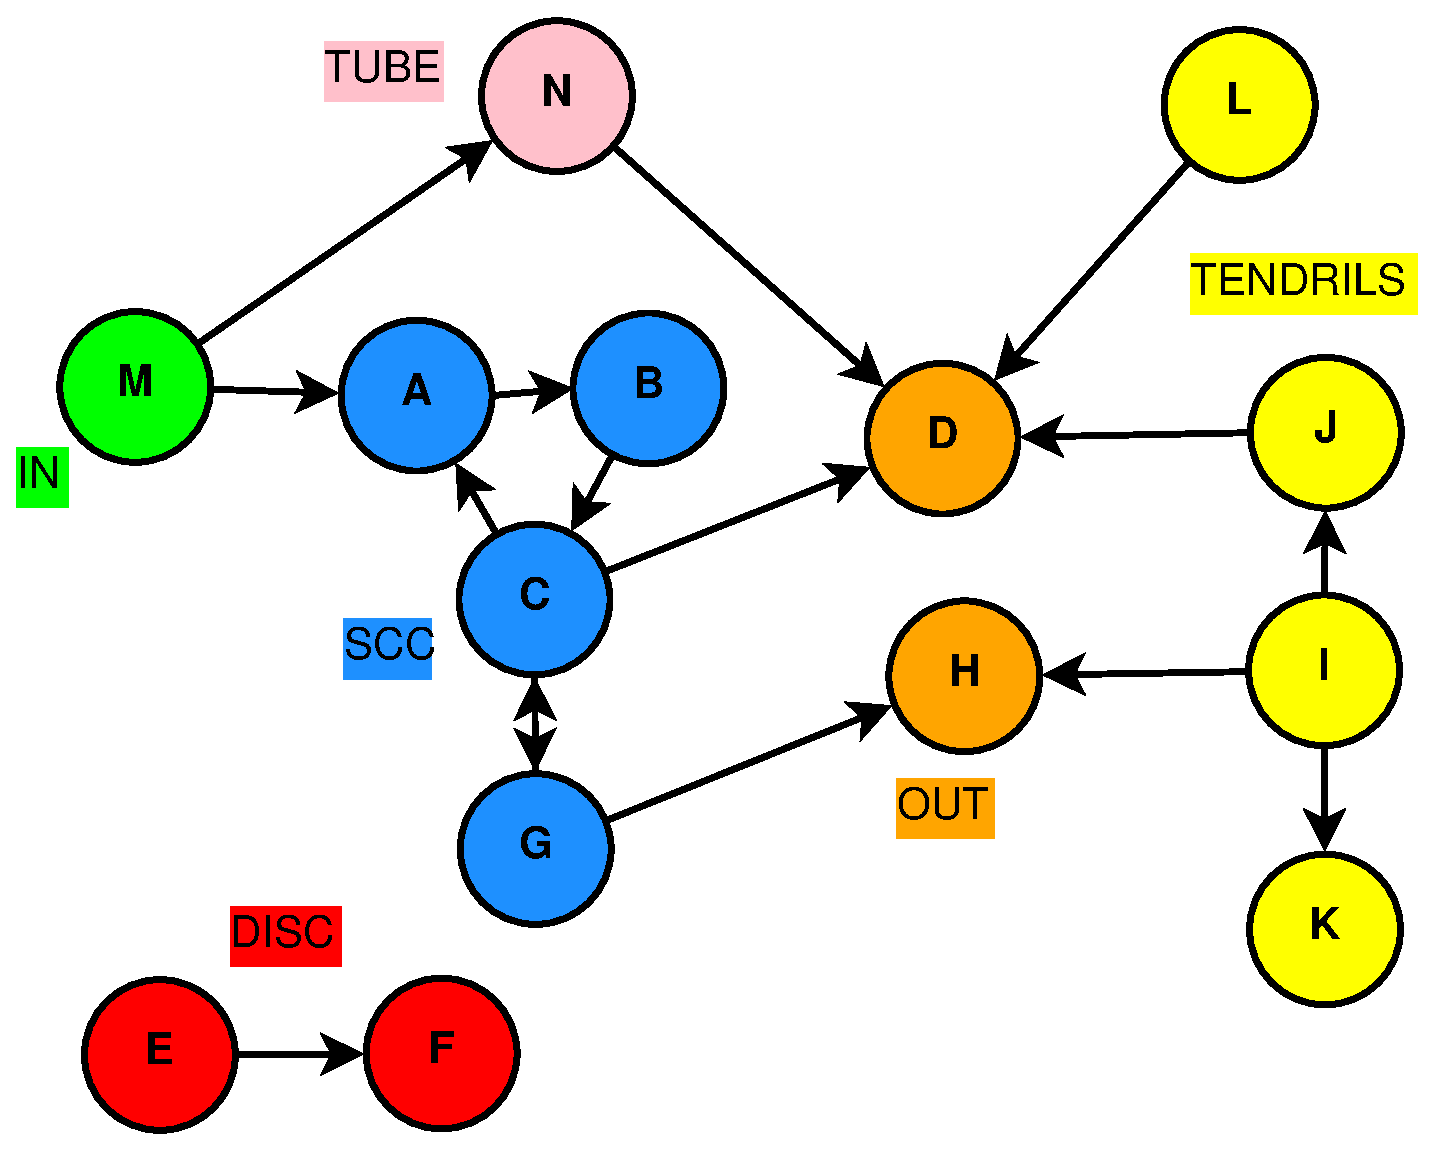
\includegraphics[width=.8\textwidth]{figures/graphLabel.eps}
	
\end{figure}


\pagebreak

\lstset{
    language=python,
    label=code:correction_8.5,
    caption={Code Listing the relevance file corrector}
}

\lstinputlisting{../q3/graphSc.py}

%%%%%%%%%%%%%%%%%%%%%%%%%%%%%%%%%%%%%%%%%%%%%%%%%%%%%%%%%%%


%%%%%%%%%%%%%%%%%%%%%%%%%%%%%%%%%%%%%%%%%%%%%%%%%%%%%%%%%%%



\begin{thebibliography}{9}

\bibitem{lamport94}\url{http://www.google.com}
\bibitem{lamport94}\url{http://jakevdp.github.io/blog/2012/10/14/scipy-sparse-graph-module-word-ladders/}
\bibitem{lamport94}\url{http://curl.haxx.se/docs/httpscripting.html}
\bibitem{lamport94}\url{http://www.crummy.com/software/BeautifulSoup/bs4/doc/}
\bibitem{lamport94}\url{http://www.rmi.net/~lutz/}
\bibitem{lamport94}\url{http://www.cs.cornell.edu/home/kleinber/networks-book/}



\end{thebibliography}



%%%%%%%%%%%%%%%%%%%%%%%%%%%%%%%%%%%%%%%%%%%%%%%%%%%%%%%%%%%



%%%%%%%%%%%%%%%%%%%%%%%%%%%%%%%%%%%%%%%%%%%%%%%%%%%%%%%%%%%



%%%%%%%%%%%%%%%%%%%%%%%%%%%%%%%%%%%%%%%%%%%%%%%%%%%%%%%%%%%




%%%%%%%%%%%%%%%%%%%%%%%%%%%%%%%%%%%%%%%%%%%%%%%%%%%%%%%%%%%



%%%%%%%%%%%%%%%%%%%%%%%%%%%%%%%%%%%%%%%%%%%%%%%%%%%%%%%%%%%




\end{document}


